
\documentclass{beamer}
\usepackage{graphicx}
\usepackage{amsmath}
\usetheme{metropolis}
\usepackage{multirow}
\usepackage{tabularx}
\usepackage{amsthm}
\usepackage{appendixnumberbeamer}
\usepackage{caption}

\hypersetup{
	colorlinks=true,
	linkcolor=blue,
	filecolor=blue,      
	urlcolor=blue,
	citecolor=blue,
}
\usepackage{natbib}
\bibliographystyle{chicago}

\theoremstyle{plain}
\newtheorem{thm}{Theorem}[section]
\newtheorem{lem}[thm]{Lemma}
\newtheorem{prop}{Proposition}
\newtheorem*{cor}{Corollary}
\newtheorem{assumption}{Assumption}


\title{Lot Sizes, Welfare and Urban Form: A View from the United States}
\author{James Macek}
\begin{document}

\begin{frame}[plain]
	\maketitle
\end{frame}

\begin{frame}
	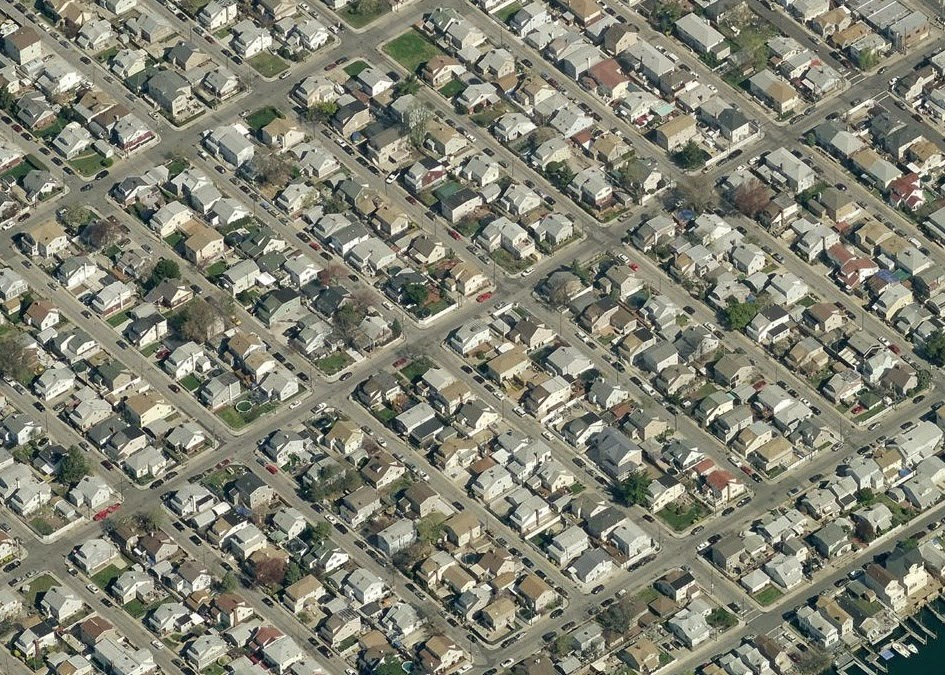
\includegraphics[width = \textwidth]{Gerritsen.jpg}
\end{frame}

\begin{frame}{Motivation}
	\begin{itemize}
		\itemsep1em
		\color{black}
		\item High housing prices in "superstar" cities are disproportionately affecting low income households \citep{albouyetal} \pause
		\item Pervasive US Housing regulation is playing a role, with real consequences for \color{red} aggregate growth \color{black} \citep{hseihmoretti} \citep{durantonpugaurbgrowth} \citep{parkho} \pause
	
		\item Lot size regulation appears to be mediating the burden of high housing prices on low income families, causing considerable \color{red} residential sorting on income \color{black} and race  \citep{kulka} \citep{Song}. \pause
		
		\item No previous work in measuring the welfare impacts in \color{red} general equilibrium\color{black}.
	\end{itemize}
\end{frame}

\begin{frame}{In this paper}
	\begin{enumerate}
		\itemsep1em
		\color{black}
		\item Income sorting has important implications for the \textit{aggregate} welfare consequences of regulation, building on \cite{hseihmoretti}:
		\begin{itemize}
			\item Deregulation causes high income, productive households to sort out of productive cities
			\item Exacerbated when local amenities are endogenous
			\item Ensuing externalities, e.g. \cite{hamilton1976}. 
		\end{itemize} \pause
		\item  Evidence that \textit{heterogeneous} regulation has altered \textit{urban form} in expensive cities. Crucial for assessing welfare consequences for two reasons:
		\begin{itemize}
			\item Households can move \textit{within} cities to avoid large lots
			\item Within-city income sorting is an important margin bolstering welfare inequality
		\end{itemize}
	\end{enumerate} 
\end{frame}

\begin{frame}{How?}
	\begin{itemize}
		\color{black}
		\itemsep1em
		\item Build and calibrate a structural GE model with heterogenous households, cities and neighborhoods across the contiguous United States
		\begin{itemize}
			\item (Heterogenous) regulations cause income sorting, and income sorting shapes the pattern of neighborhood amenities
			\item \dots and also shape patterns of urban density in a way that matches observation
		\end{itemize} \pause
		\item Counterfactual: What if we decreased the lot size restrictions we observe in the suburbs of expensive cities? \pause
		\item Housing regulation is hard to measure, but recent advances...
		\begin{itemize}
			\item \cite{Song} shows that a structural break detection algorithm works well for minimum lot sizes
			\item I hope to leverage assessment data with nation-wide coverage
		\end{itemize}
	\end{itemize}
\end{frame}


\begin{frame}{Literature}
	\fontsize{8pt}{7.2}	
	\begin{itemize}
		\itemsep1em		
			
		\item \color{red} Macroeconomics of housing regulation \citep{hseihmoretti} \citep{durantonpugaurbgrowth} \citep{parkho} \citep{bunten} \citep{hop} \citep{ganongshoag} \citep{superstarcities} 


		\item \color{red} Lot Size/Unit density regulation \citep{kulka} \citep{Song} \citep{KSC} \citep{zabel} \citep{gyourko2021} \citep{griesonwhite} \citep{gyourkovoith1997} \citep{davidoff2022}
		
		\item \color{red} Housing Regulation + Supply + Affordability \citep{BSH} \citep{saiz2010} \citep{asquithetallocaleffects} \citep{mastwarding} \citep{albouyetal} \citep{bbheight} \citep{mills2005} \citep{bruecknersingh} \citep{BruecknerFuGu} \citep{acosta} \citep{martynov} \citep{turner2014} \citep{gyourkomolloy}
		
		\item \color{purple} Urban spatial sorting \citep{diamond2016} \citep{couturehandbury} \citep{su2021} \citep{bshartley2020} \citep{Coutureetal} \citep{AlmagroDI} \citep{parispoor} \citep{ccpoortransport} \citep{Gentrificationcycles} \cite{LeeandLin}
		
		\item \color{purple} Inequality in cities \citep{ineqcitysize} \citep{spatialsorting} \citep{FogliGuerrieri}
		
		\item \color{teal} Exclusionary Zoning \citep{Hamilton1975} \citep{calabresetal} \citep{keepingpeopleout} \citep{ineffTiebout} \citep{barcoate} \citep{brueckner2021}
	\end{itemize}
\end{frame}

\section{Motivating evidence}

\begin{frame}{Fact 1: Density Gradients Differ in Expensive Cities}
\begin{itemize}
	\itemsep1em
	\color{black}
	\item Using tract level data from the 2010 Census \pause
	\item Within each 2013 MSA, I rank tracts by their density of housing units. Ranking lies in the unit interval. \pause
	\item I flexibly regress tract-level housing unit density against this ranking separately for both the "Superstar" and "Non-Superstar" samples. \pause
	\item Superstars are MSAs in the top quartile of (unadjusted) housing prices, Non-superstars in the bottom quartile \pause
	\item Housing unit density is \color{red} normalized to be on average 1 \color{black} across tracts within each MSA. Controls for MSA fixed effects. 
\end{itemize}
\end{frame}

\begin{frame}{Fact 1: Density Gradients Differ in Expensive Cities}
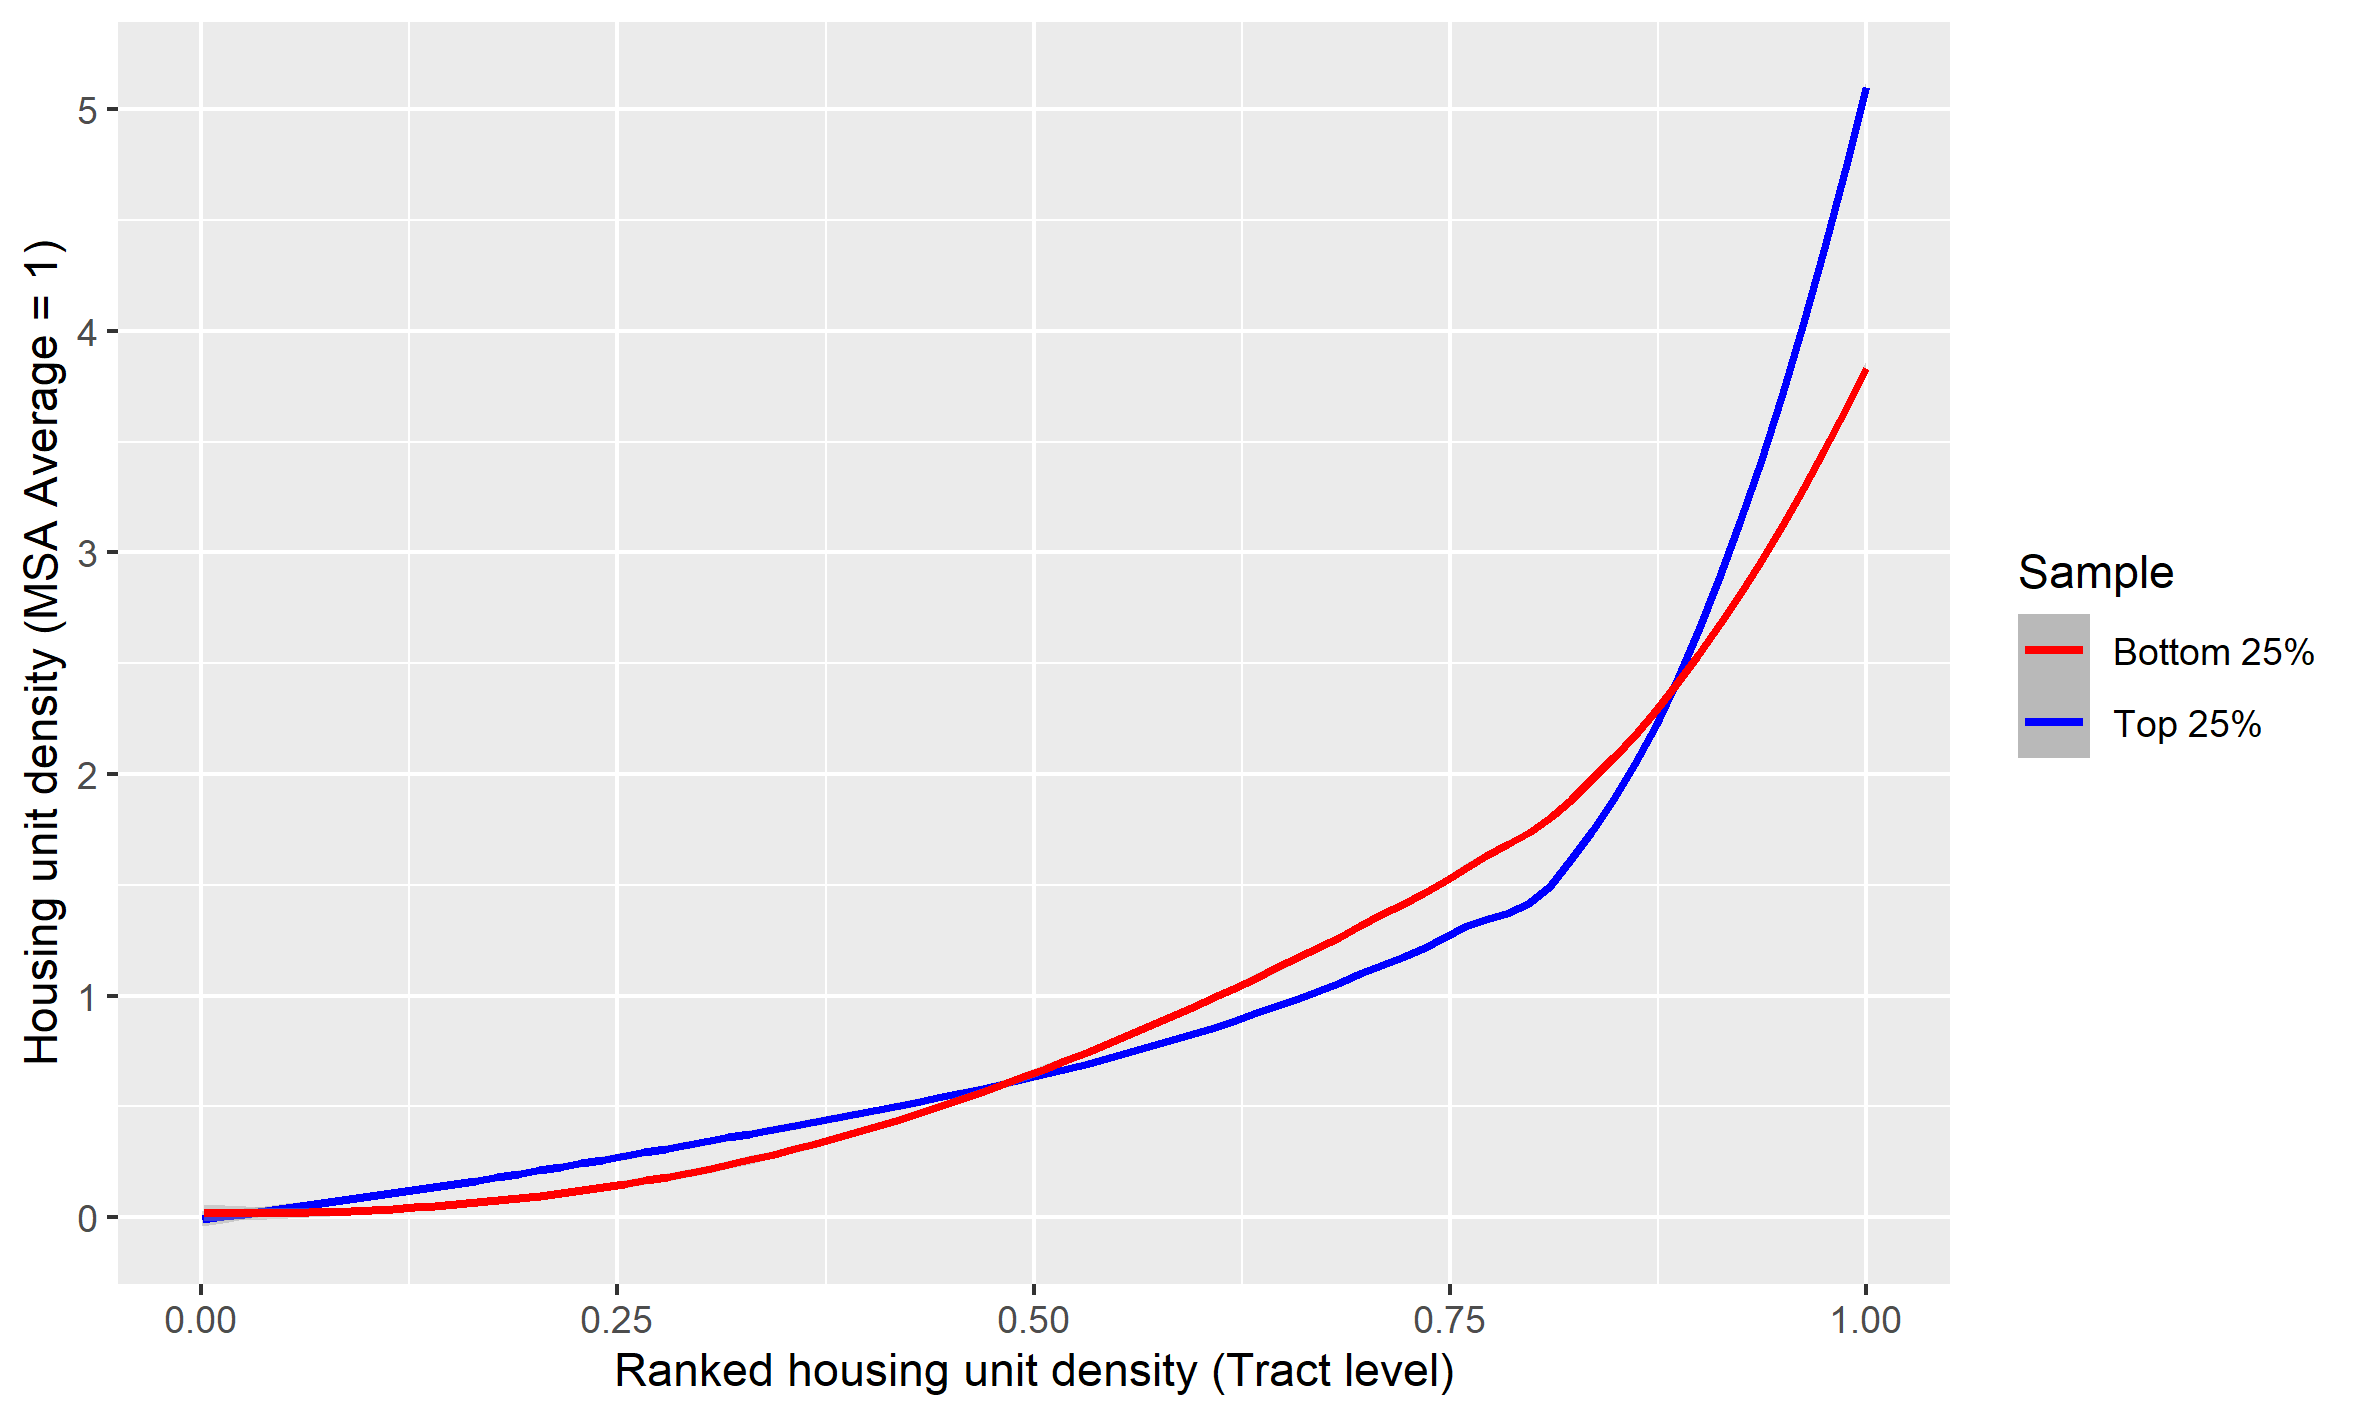
\includegraphics[width=\textwidth]{tractdens_dist.png}
\end{frame}

\begin{frame}{Fact 1: Why might lot size regulation be generating these patterns?}
\begin{enumerate}
	\label{return}
	\itemsep1em
	\color{black}
	\item Decompose Housing Unit Density into a \color{red} \textit{Single Family} \color{black} margin and an \color{red} \textit{Other Structures} \color{black} margin \hyperlink{1}{\beamerbutton{Go!}} 
	
	\item Further decompose Single Family margin into \color{red} \textit{Land} \color{black} and  \color{red} \textit{Density} \color{black} margins, using assessment data \hyperlink{2}{\beamerbutton{Go!}} 
	
	\item Fact 1 does \color{red} \textit{not} \color{black} replicate in contemporary French cities \hyperlink{3}{\beamerbutton{Go!}} 
	
	\item TBD: Does Fact 1 replicate in the early 20th century US? 
\end{enumerate}
	
\end{frame}


\begin{frame}{Fact 2: Strong Income Sorting on Density in Expensive Cities}
	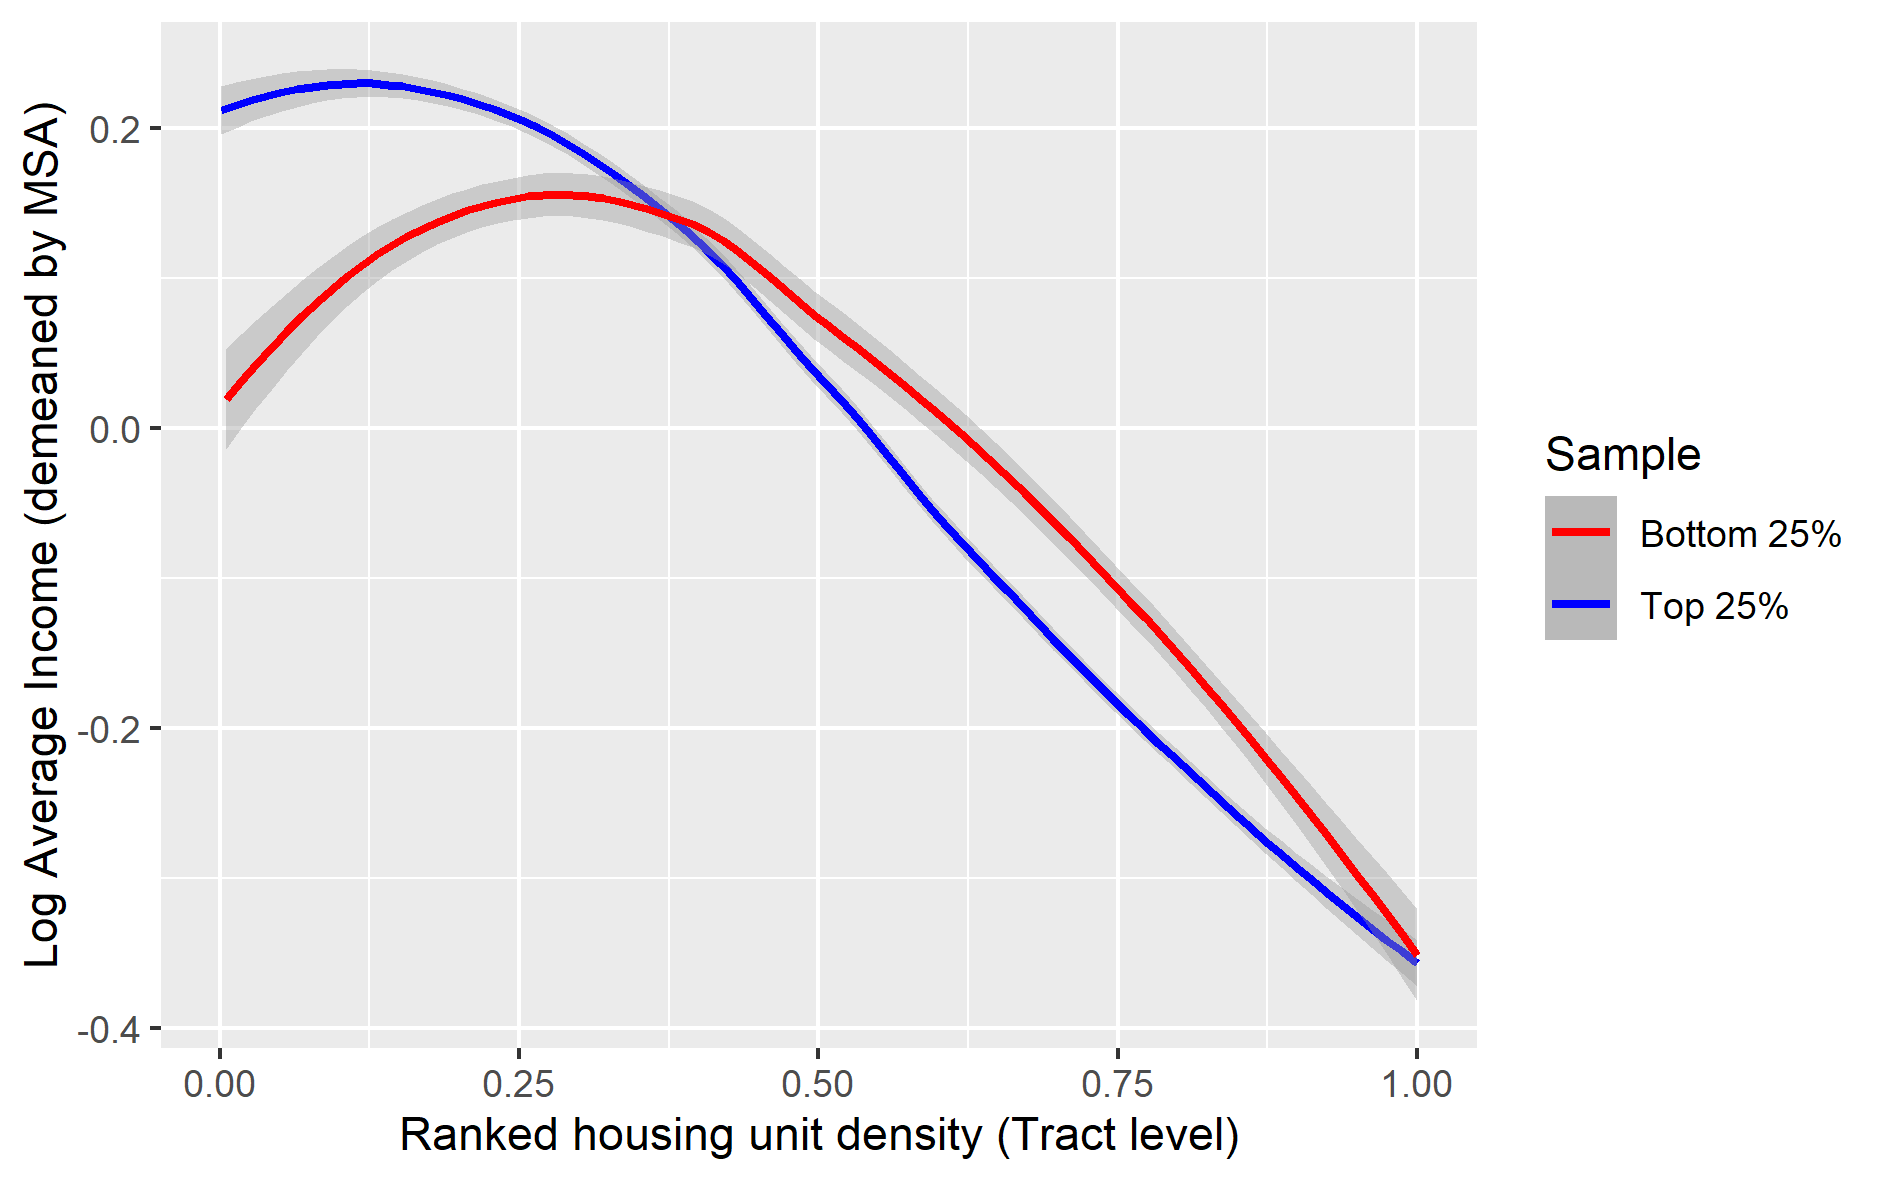
\includegraphics[width= \textwidth]{income.png}
\end{frame}

\section{Model and Calibration}
\begin{frame}{Preliminaries}
	\begin{itemize}
		\color{black}
		\itemsep1em
		\item Let $i$ index a particular 2010 census tract; will be the definition of a \textit{neighborhood} in the model.  \pause
		
		\item Let $C(i)$ be the 2013 MSA associated with $i$ \pause
		
		\item Let $N(c)$ be the set of neighborhoods contained in MSA $c$ \pause
		
		\item Unless otherwise stated, all data are from the 2010 Census or the 2008-2012 ACS, where applicable. \pause
		
		\item Each tract $i$ has land $T(i)$ available for residential  development.  
	\end{itemize}
\end{frame}


\begin{frame}{Developer's Problem}
	\begin{itemize}
		\color{black}
		\item Start with a standard Cobb-Douglas production function for housing, yielding housing supply per unit of land
		\begin{equation}
		A(i) = \bigg[\frac{P(i)}{\lambda(i)}\bigg]^{\epsilon(i)}
		\end{equation} \pause
		
		
		\item Minimum lot sizes complicate things. Developers need to \color{red}\textit{respect the allocation of housing stock across housing units}\color{black}.
		
		\item Minimum lot sizes $l(i)$ incentivize developers to build above a \textit{minimum housing stock per housing unit}   \pause
		\begin{equation}
			A^{\star}(i) = \bigg[\frac{P(i)}{\lambda(i)}\bigg]^{\epsilon(i)}l(i)
		\end{equation}
	\item Note: $P(i)A^{\star}(i)$ is increasing in $P(i)$. 
	\end{itemize}
\end{frame}

\begin{frame}{Consumer's Problem}
	\begin{itemize}
		\color{black}
		\itemsep1em
		\item Suppose a household chose neighborhood $i$ in city $C(i)$: \pause
		\item Household differs on effective units of labour $z \in Z$, receive a city specific wage $w(c)$ and a neighborhood-type amenity $b(i, z)$ \pause
		\item Household has Cobb Douglas preferences over housing $A$ and numeraire good $g$
		\begin{equation}\label{utility}
			\max_{A, g} b(i, z)A^{\beta}g^{1-\beta}
		\end{equation} 
		subject to \color{red}$A \geq A^{\star}(i)$ \color{black} and $P(i)A + g \leq w(i)z$. \pause
		
		\item Let $V\big[P(i), w(i), z, A^{\star}(i)\big] := V(i, z)$ be the indirect utility associated with this problem. 
	\end{itemize}
		
\end{frame}

\begin{frame}{Neighborhood Choice}
	\begin{itemize}
		\color{black}
		\item Frechet shocks over neighborhoods, allowing for within-city correlation $\rho$. Labour supply for type $z$ households are 
			\begin{equation}\label{laboursupply}
				L(i, z) = \bigg[\frac{W(C(i), z)}{\boldsymbol{W}(z)}\bigg]^{\theta}\bigg[\frac{V(i, z)}{W(C(i), z)}\bigg]^{\frac{\theta}{1-\rho}}\bar{L}(z)
		\end{equation}
		\pause with 
		 \begin{equation*}
			W(C(i), z) = \bigg[\sum_{i' \in N\big[C(i)\big]}V(i', z)^{\frac{\theta}{1-\rho}}\bigg]^{\frac{1-\rho}{\theta}}
		\end{equation*} 
		\pause and
		\begin{equation*}
			\boldsymbol{W}(z) = \bigg[\sum_{c \in C} W(c, z)^{\theta}\bigg]^{\frac{1}{\theta}}	
		\end{equation*}
	\end{itemize}
\end{frame}

\begin{frame}{Endogenous Amenities}
	\begin{itemize}
		\color{black}
		\itemsep1em
		\item  Let $\tau(i)$ be the commuting time in $i$. I allow amenity values $b(i, z)$ to respond to neighborhood income per capita via the equation:
		\begin{equation}
			 	\log\big[b(i, z)\big] = -\kappa\tau(i) + \Omega\log\bigg[\frac{\sum_{z' \in Z}w(i)z'L(i, z')}{\sum_{z' \in Z}L(i, z')}\bigg] + \epsilon(i, z)
		\end{equation} \pause
	\item Two microfoundations 
	\begin{enumerate}
		\itemsep1em
		\item Local, non-traded Dixit-Stiglitz market  \citep{Coutureetal} \citep{AlmagroDI} + local disutility of density \citep{KSC} \pause
		\item Local, congested public good financed through property taxes \citep{calabresetal} \citep{ineffTiebout}
	\end{enumerate}
	\end{itemize}
\end{frame}

\begin{frame}{Wages}
	\begin{itemize}
		\color{black}
		\itemsep1em
		\item Numeraire good is produced using only units of labour under \textit{external increasing returns}.
		\item Inverse labour demand given by
		\begin{equation}
			w(c) = \sigma(c)\bigg[\sum_{z \in Z}\sum_{i \in N(c)}zL(i, z')\bigg]^{\alpha}
		\end{equation}
	for $\alpha > 0$.
	\item Past literature estimates $\alpha$ as a population elasticity, but with heterogenous households this interpretation is lost. 
	\item Apparently, hard to separately identify agglomeration effects on output and population, See \cite{Agglomerationemp} Section 3.1. 
	\end{itemize}
\end{frame}

\section{Calibration and Identification}

\begin{frame}{Minimum Lot Sizes}
	\begin{itemize}
		\color{black}
		\itemsep1em
		\item Follows a structural break algorithm in \cite{Song}.
			\begin{itemize}
				\item Idea: Zoning variances are present, but rare
				\item Implies "bunching" of lot sizes around the minimum 
				\item Can be fit with a discontinuous CDF after constructing "zoning districts" in a data driven way
			\end{itemize} \pause
		
		\item I generalize this procedure to multifamily homes (duplexes, triplexes and fourplexes)
		
		\item Problem: Lot size policy may vary within census tracts. 
		\begin{itemize}
			\item If multiple minimum lot sizes overlap on a tract, consider the smallest one
			\item Assign the measured minimum lot size to a tract if the observed number of housing units does not exceed the \textit{implied} maximum under regulation. 
		\end{itemize}
	\end{itemize}
\end{frame}

\begin{frame}{Regional Production Functions}
	\begin{itemize}
		\itemsep1em
		\color{black}
		\item Follows \cite{BSH} closely, with some differences
		\begin{enumerate}
			\item Use assessment data to construct high quality measures of housing prices $P(i)$ via a hedonic regression
			\item Use the most general definition of housing services. That is, the measure of housing stock on some lot is its value deflated by $P(i)$.  \pause
		\end{enumerate}
		\item Given stock measures $A(i)$, prices $P(i)$ and elasticities $\epsilon(i)$ from \cite{BSH}, supply shifters $\lambda(i)$ are uniquely identified \dots
		\item and so is the minimum housing stock per unit $A^{\star}(i)$
	\end{itemize}
\end{frame}

\begin{frame}{Recovering Amenities $b(i, z)$}
	\begin{itemize}
		\color{black}
		\itemsep1em
		\item Use a Mincer regression with MSA fixed effects to decouple city and individual productivity. \pause
		\item Local income distributions are observed in the ACS, and are then transformed to local distributions of $z$ 
		\begin{itemize}
			\item Choose $b(i, z)$ to rationalize this data after accounting for model-implied consumption
			\item Fix value $\kappa = 0.01$ from \cite{berlinwall} \pause
		\end{itemize}
		\item For now: choose a value of $\theta$ and $\rho$ from the literature
		\begin{enumerate}
			\item \cite{morettihornbeck} measure $\theta \approx \frac{10}{3}$
			\item \cite{herzog2022} estimates $\frac{\theta}{1-\rho} = 7.21$ in a closed city model of commuting, implying $\rho \approx 0.5377$ 
		\end{enumerate}
	\end{itemize}

\end{frame}

\begin{frame}{Estimation of $\Omega$}
	\begin{itemize}
		\color{black}
		\itemsep1em
		\item Recall the estimating equation: 
		\begin{equation*}
			\log\big[b(i, z)\big] = -\kappa\tau(i) + \Omega\log\bigg[\frac{\sum_{z' \in Z}w(i)z'L(i, z')}{\sum_{z' \in Z}L(i, z')}\bigg] + \epsilon(i, z)
		\end{equation*} \pause
		\item Two sources preventing identification:
		\begin{enumerate}
			\item Simultaneity bias, analogous to \cite{Coutureetal} and \cite{diamond2016}.
			\item Exogenous, unobserved features that cause amenities and income sorting, \color{red} but do not respond to changes in local incomes\color{black}. 
		\end{enumerate}
	\end{itemize}
\end{frame}

\begin{frame}{Estimation of $\Omega$}
 \begin{itemize}
 	\color{black}
 	\itemsep1em
 	\item I propose an instrument -- tract level terrain slopes. There are two competing interpretations of its validity:
 	\begin{itemize}
 		\color{black}
 		\item \cite{saiz2010}: Slopes primarily affect housing prices through \textit{supply constraints}. \color{blue} Validates the instrument\color{black}.
 		\item \cite{LeeandLin}: Slopes primarily affect housing prices through \textit{amenities}. \color{red} Invalidates the instrument\color{black}.
 		
 	\end{itemize} \pause
 	\item To address the amenities interpretation, I control for a large set of observed local amenities from \cite{LeeandLin} and the National Land Cover Database + MSA Fixed Effects \pause
 	\item For most amenities variables $v_{i}$ and average slope $s_{i}$, I construct an additional control $v_{i}s_{i}$
 	\begin{itemize}
 		\item Accounts for supermodularities between slopes and natural features
 		\item Example: can have an ocean view from farther away if terrain is sloped
 	\end{itemize} 
 \end{itemize}
\end{frame}

\begin{frame}{Estimation of $\Omega$: First Stage}
	\color{black}
	\begin{figure}
		\centerline{\resizebox{12cm}{3cm}{\begin{tabular}{lccc} \hline
 & (1) & (2) & (3) \\
VARIABLES & Log(Average Income) & Log(Average Income) & Log(Average Income) \\ \hline
 &  &  &  \\
Average Slope & 0.022*** & 0.024*** & 0.010 \\
 & (0.002) & (0.004) & (0.012) \\
 &  &  &  \\
Observations & 58,498 & 58,350 & 58,350 \\
R-squared & 0.038 & 0.007 & 0.000 \\
KP F-Stat & 100.397 & 35.884 & .588 \\
MSA FE & Yes & Yes & Yes \\
MSA Clustering & Yes & Yes & Yes \\
 Amenity Controls & No & Yes & Yes incl. slope x max july temperature \\ \hline
\multicolumn{4}{c}{ Robust standard errors in parentheses} \\
\multicolumn{4}{c}{ *** p$<$0.01, ** p$<$0.05, * p$<$0.1} \\
\end{tabular}
}}	
	\caption{\scriptsize Amenity Controls: A set of approximately 240 variables, merging data from \cite{LeeandLin} and measures of forest and perennial snow cover from the NLCD. \cite{LeeandLin} controls include distance to various bodies of water, temperature, precipitation, different types of community names (i.e. "gulch", "shores"). Includes most interactions of these variables with average slopes.}
	\end{figure}	
\end{frame}

\begin{frame}{Conclusion}
	\begin{itemize}
		\color{black}
		\itemsep1em
		
		\item I provide observational evidence that \textit{heterogeneous} lot size regulation has altered urban form -- both the shape of cities and how households of various incomes sort into them.
		
		\item Income sorting in the face of lot size regulation has important implications for aggregate welfare.
		
		\begin{itemize}
			\item A channel that has been (sadly) ignored. 
		\end{itemize}
		 
		
		\item This motivates a structural model that can simultaneously capture all these forces. 
		
		\item Thank you for all the help this year!
	\end{itemize}
\end{frame}


\section{Appendix}
\appendix
\begin{frame}{Appendix: Single Family Margin vs Other Structures}
\begin{itemize}
\color{black}
\item The shape of the distribution \textit{may not} be driven the presence of structures that tend to be heavily regulated. 
\item Linearly decompose housing unit density $D_{H, im}$ into two margins:
\begin{equation}
	D_{H, im} = D_{S, im} + D_{L, im}
\end{equation}
\item where $D_{S, im}$ is the number of single family homes in MSA $m$ and tract $i$ divided by the total land mass of the tract. 
\item $D_{L, im}$ are defined analogously for all other structures. 

\item Single family home shares are from the 2008-2012 ACS. 

\item \color{red} Repeat \color{black} the regression for each component separately. Justified because the conditional expectation is additive.
\end{itemize}
\end{frame}

\begin{frame}{Appendix: Single Family and Other Structures margins 	\hyperlink{return}{\beamerbutton{Return!}} }\label{1}
	\centerline{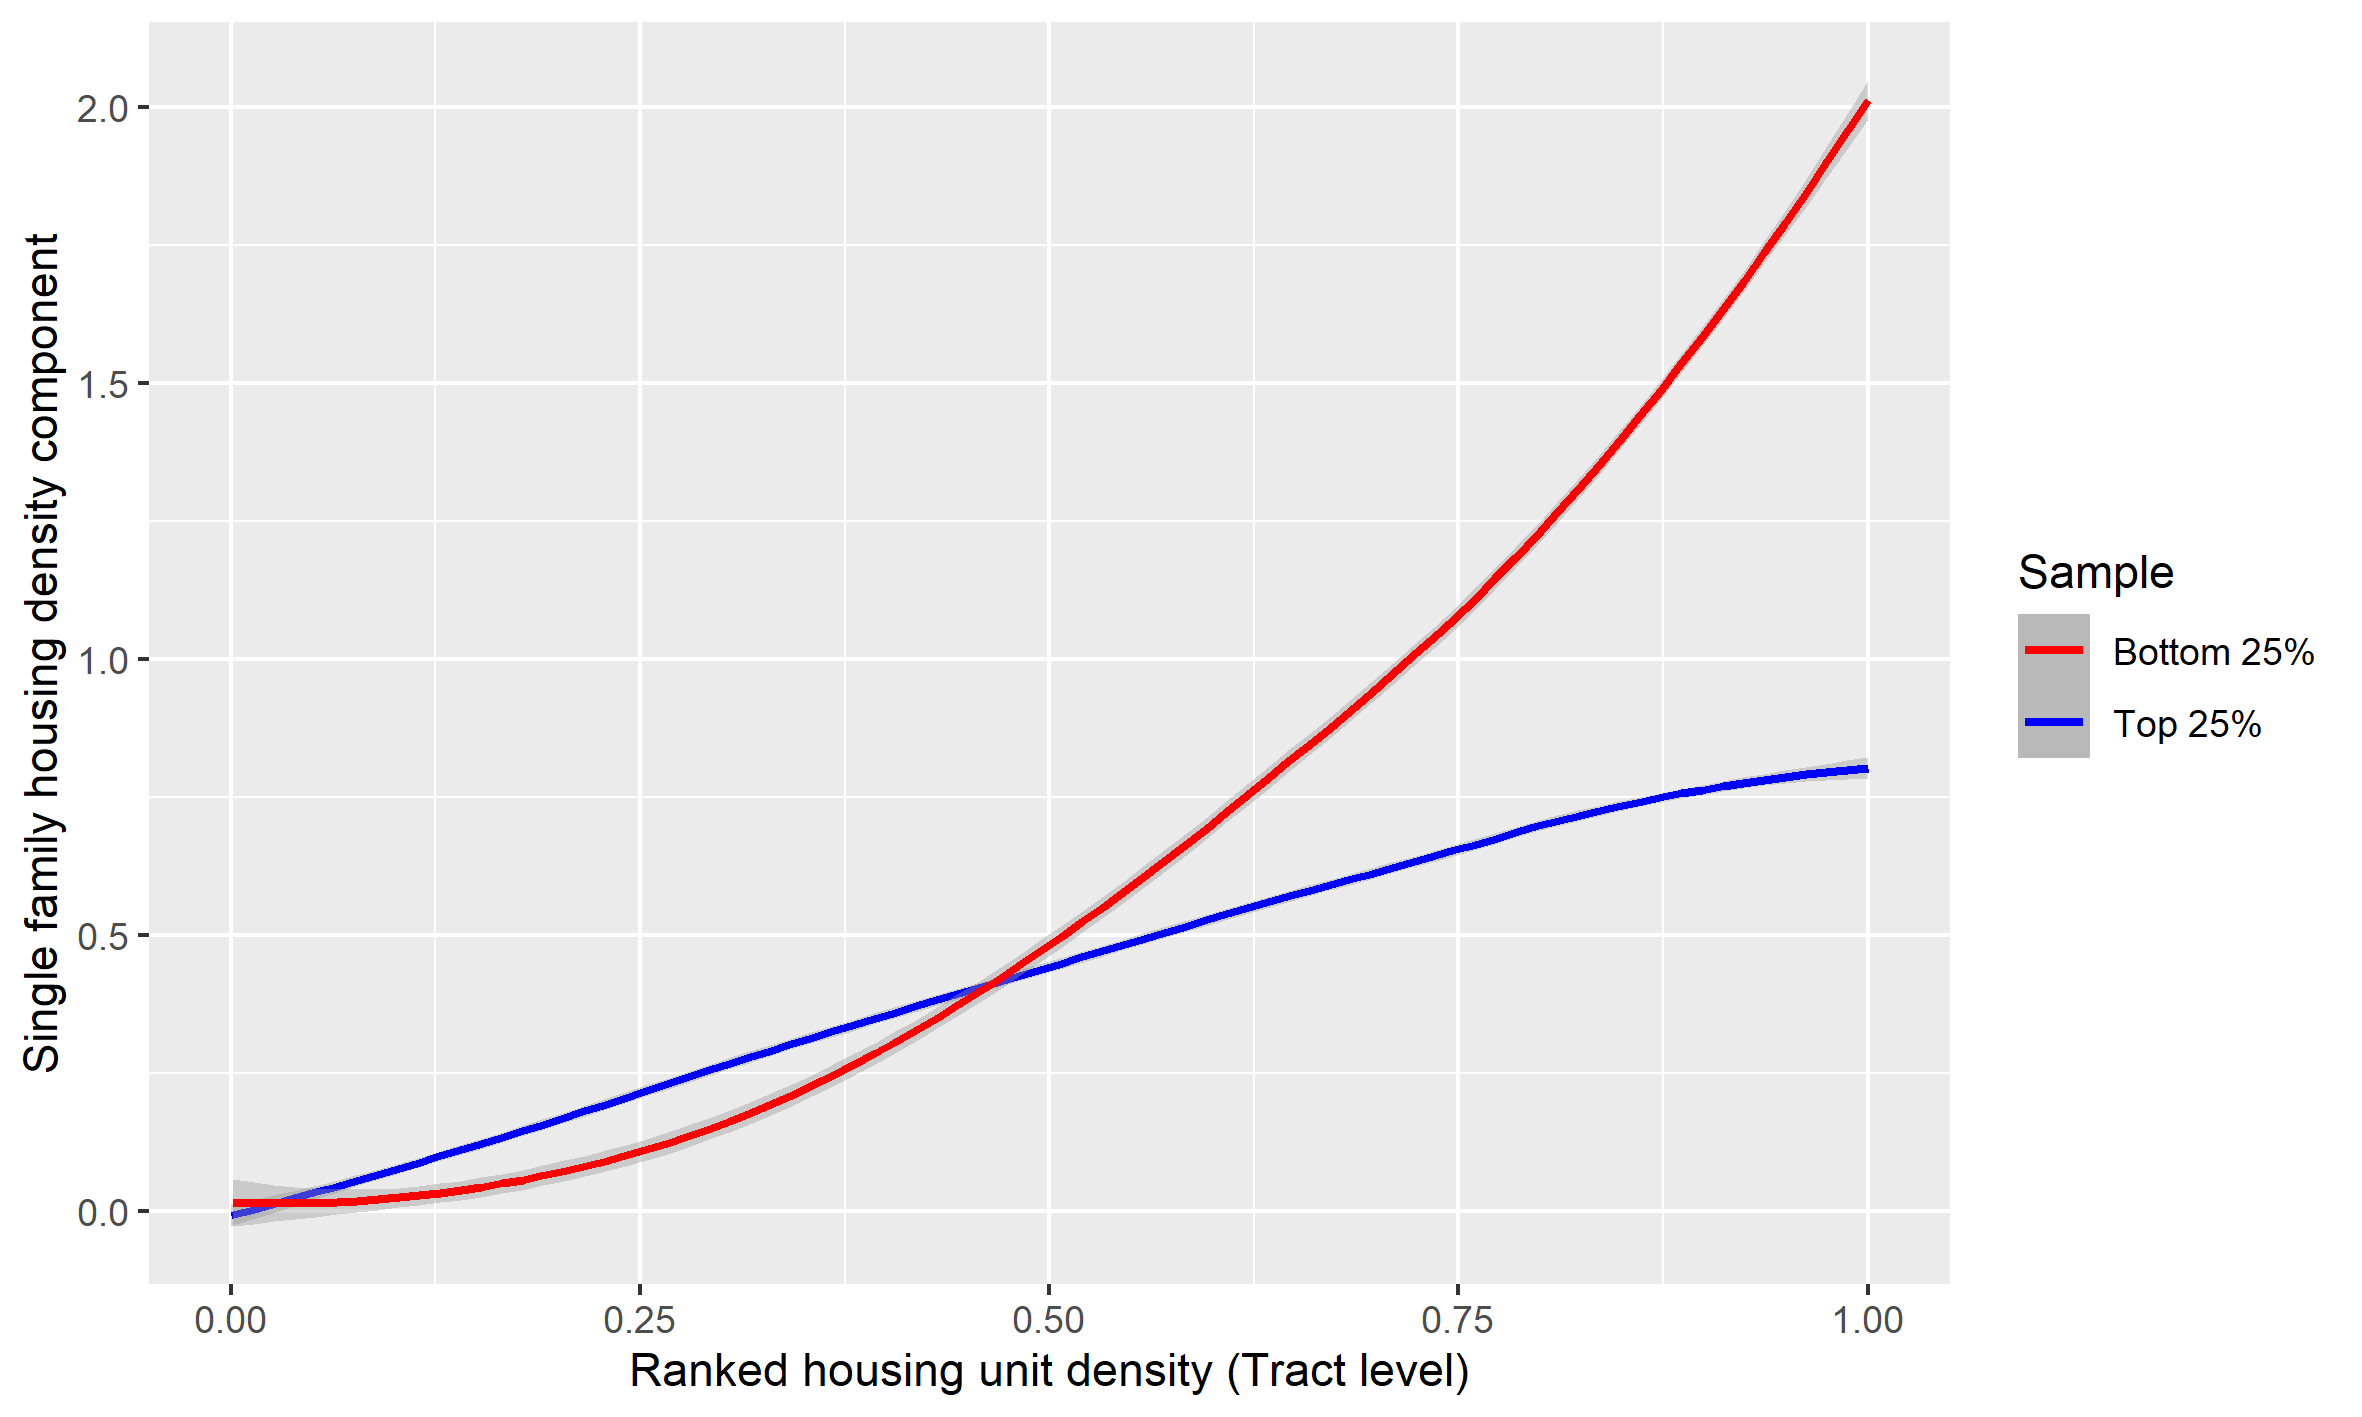
\includegraphics[width=0.7\textwidth, height=0.5\textheight]{singlefamily_dist.png}}
	\centerline{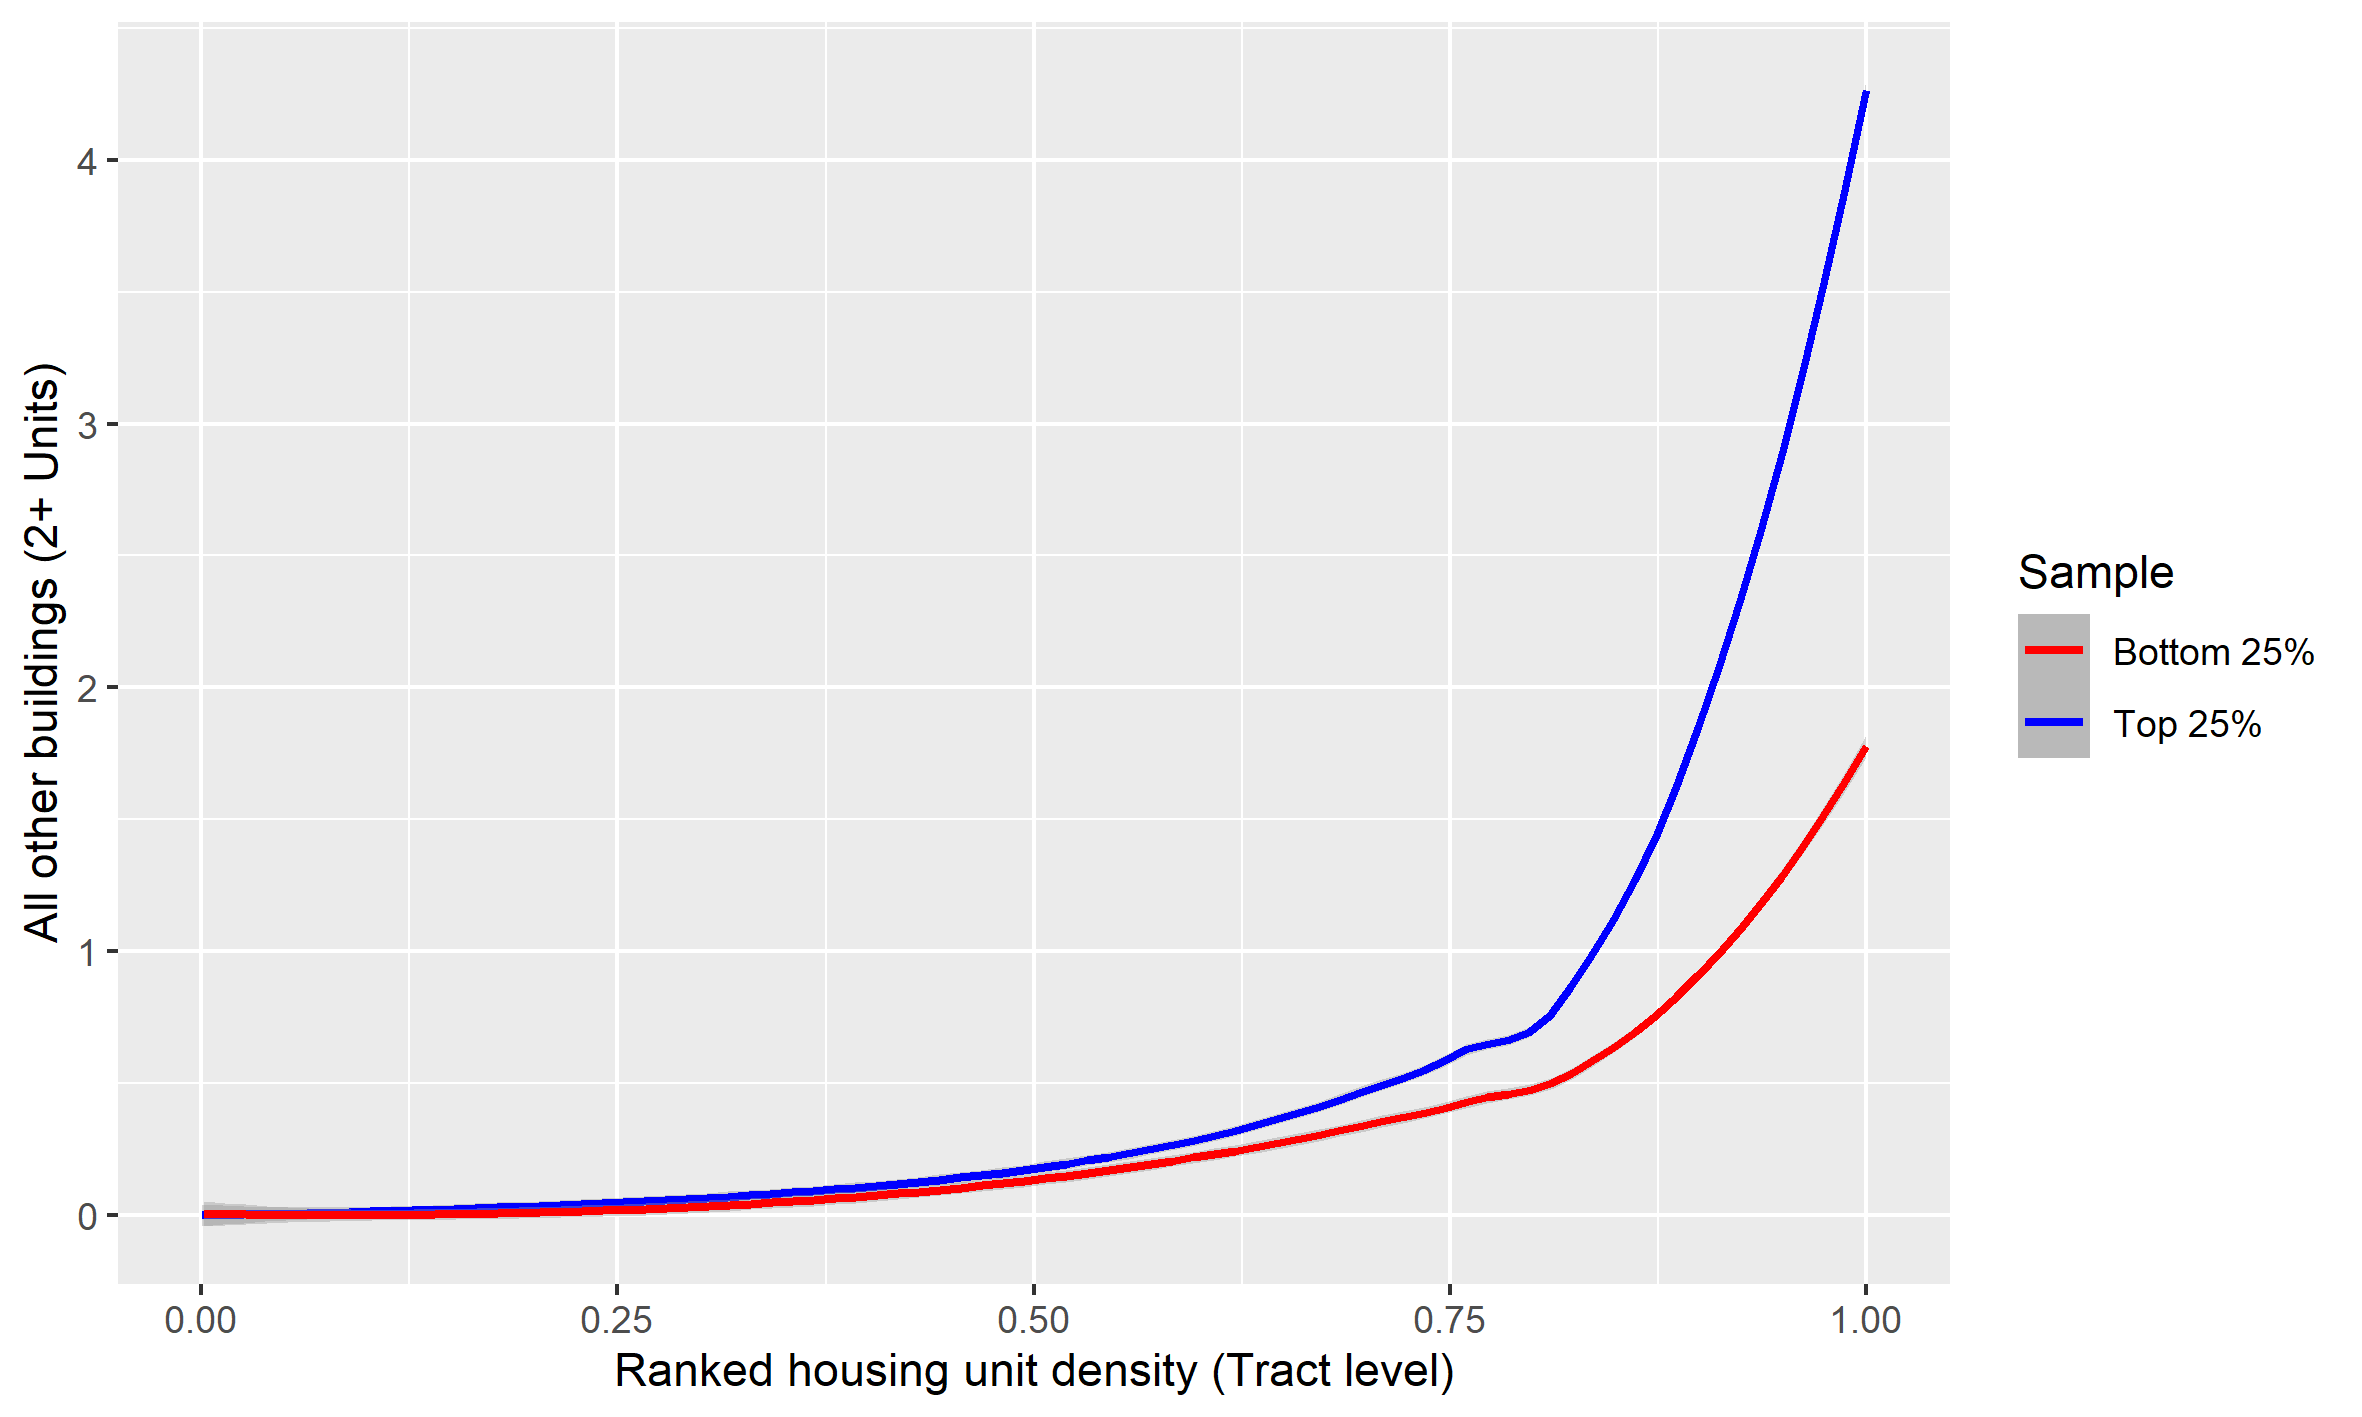
\includegraphics[width=0.7\textwidth, height=0.5\textheight]{2plusbuilding_dist.png}}

\end{frame}

\begin{frame}{Appendix: Single Family Density and Land margins}
\begin{itemize}
	\itemsep1em
	\color{black}
	\item Log-linearly decompose the single family component into \textit{density} and \textit{land} margins, respectively: 
	\begin{equation}
		log(D_{S, im}) = log(\tilde{D}_{S, im}) + log(L_{S, im})
	\end{equation}
	\item where $\tilde{D}_{S, im}$ is the number of single family homes divided by the total land used for single family housing, and $L_{S, im}$ is the fraction of tract land used for single family housing. 
	\item \color{red} Repeat the regression for each component separately. \color{black}
	\item Use 2015 assessment data on single family homes to measure average land use per housing unit, with unit counts from the ACS/Census.  
\end{itemize}
\end{frame}

\begin{frame}{Appendix: Single Family Density and Land margins \hyperlink{return}{\beamerbutton{Return!}} }
	\label{2}
	\centerline{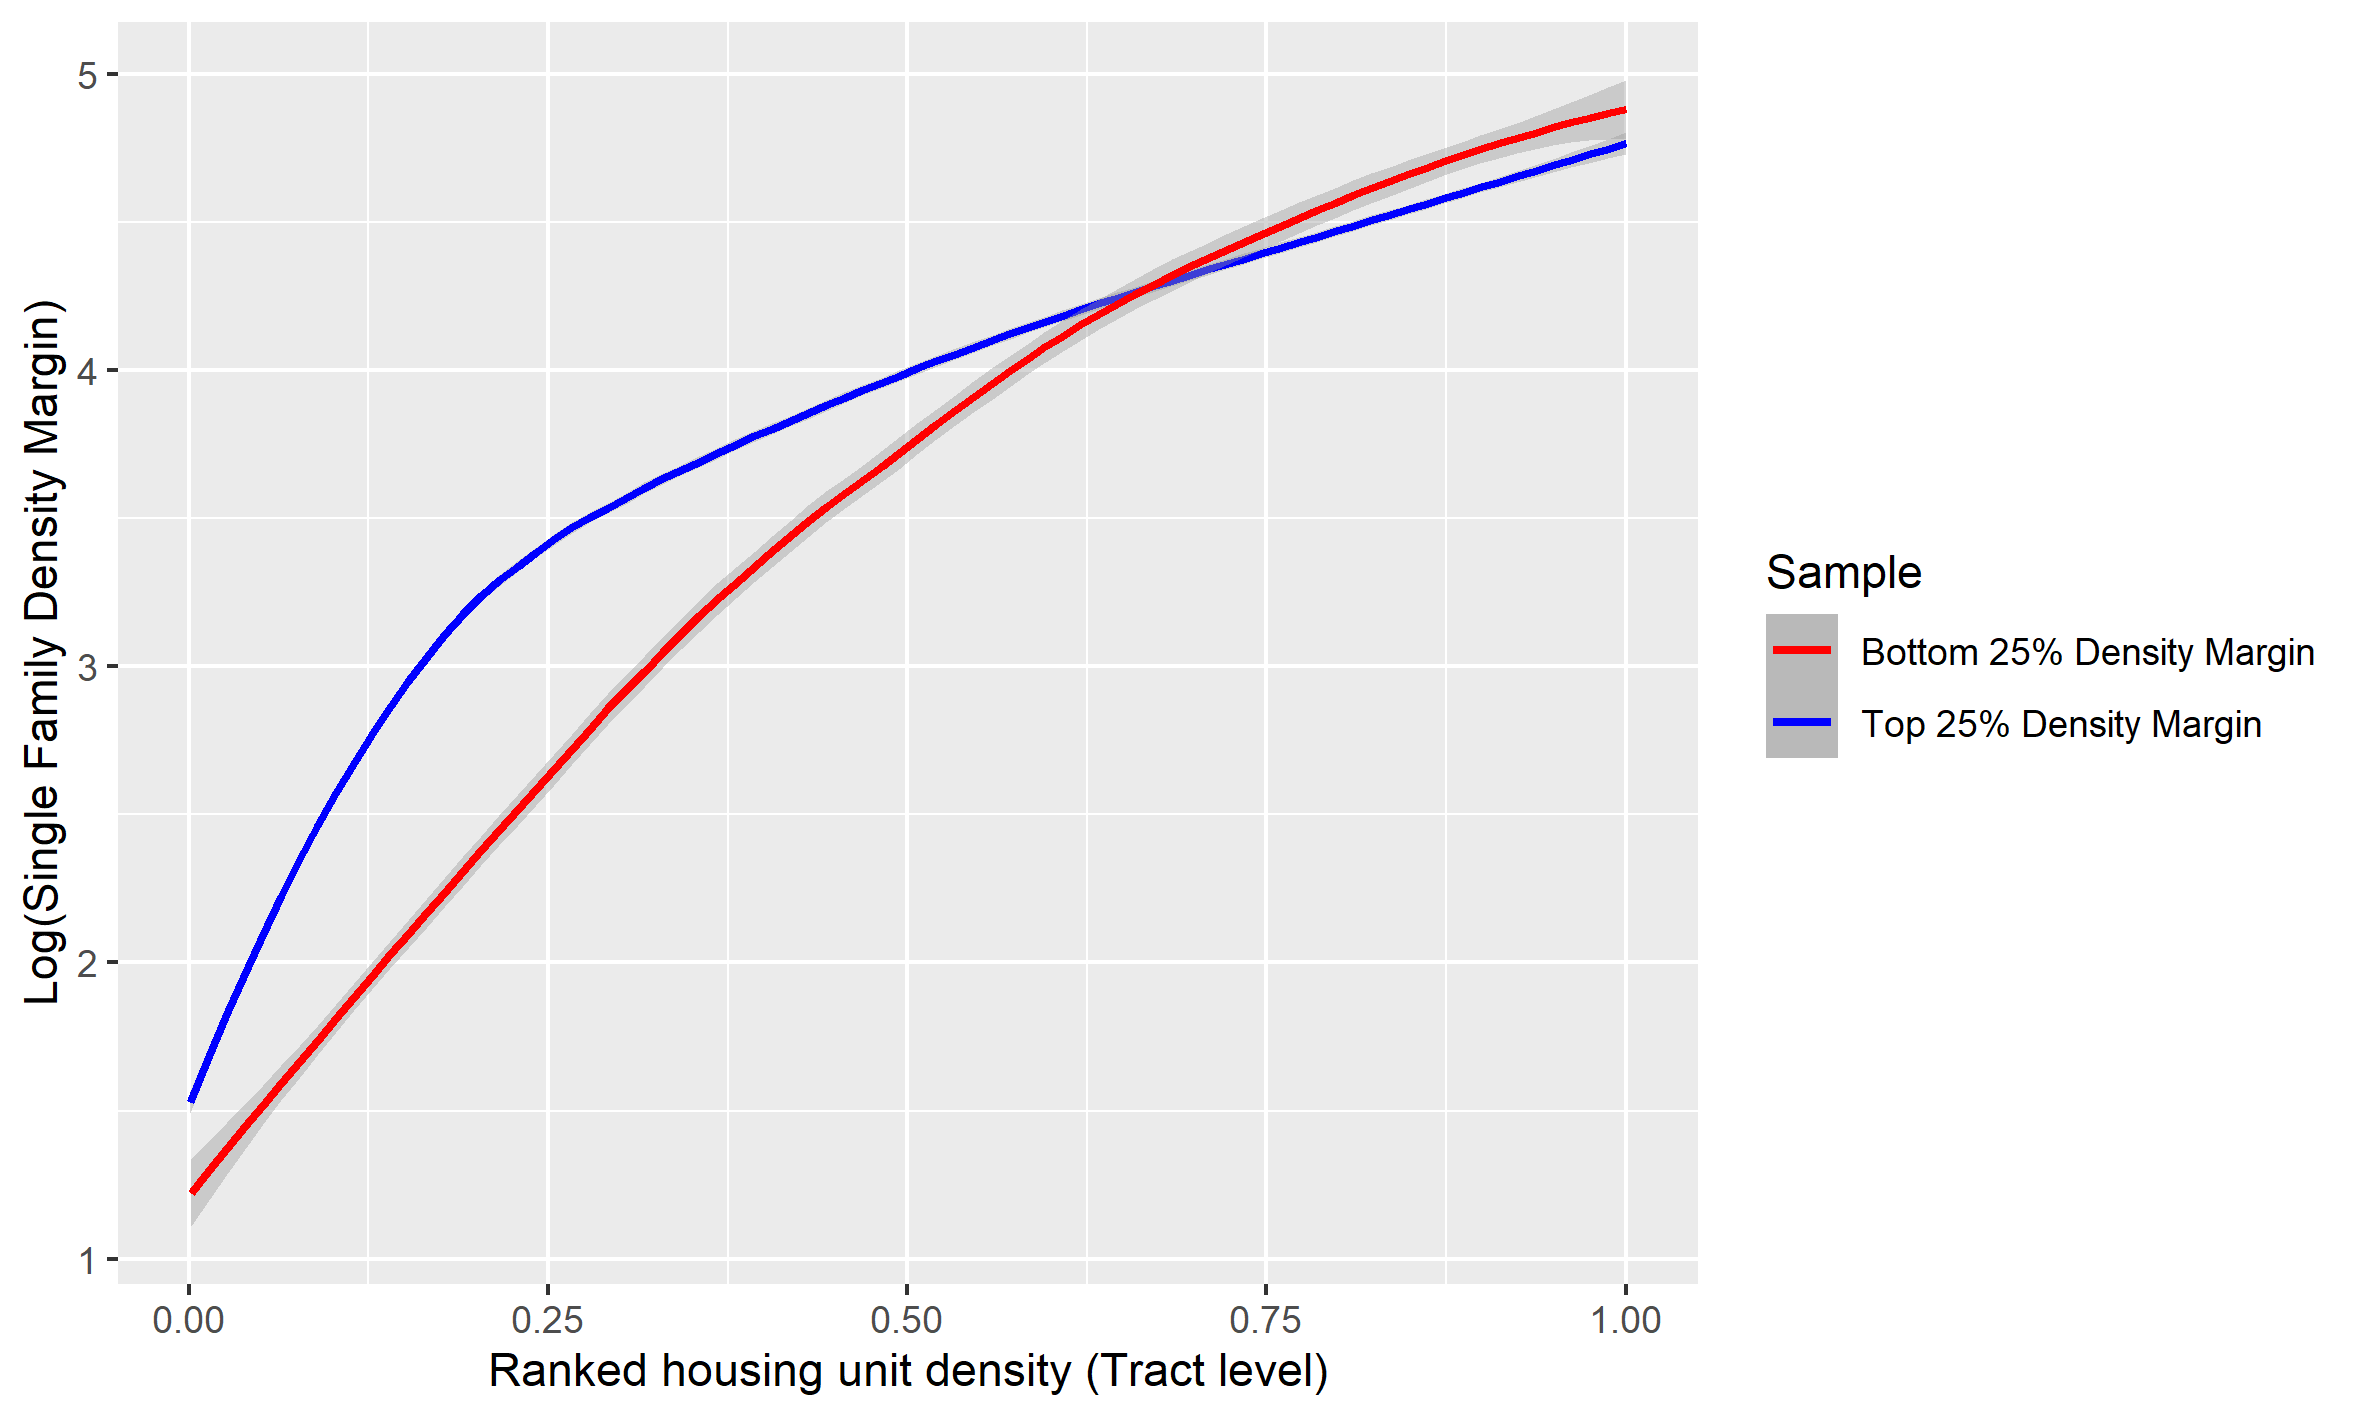
\includegraphics[width=0.7\textwidth, height=0.5\textheight]{SingleFamilyDensity.png}}
	\centerline{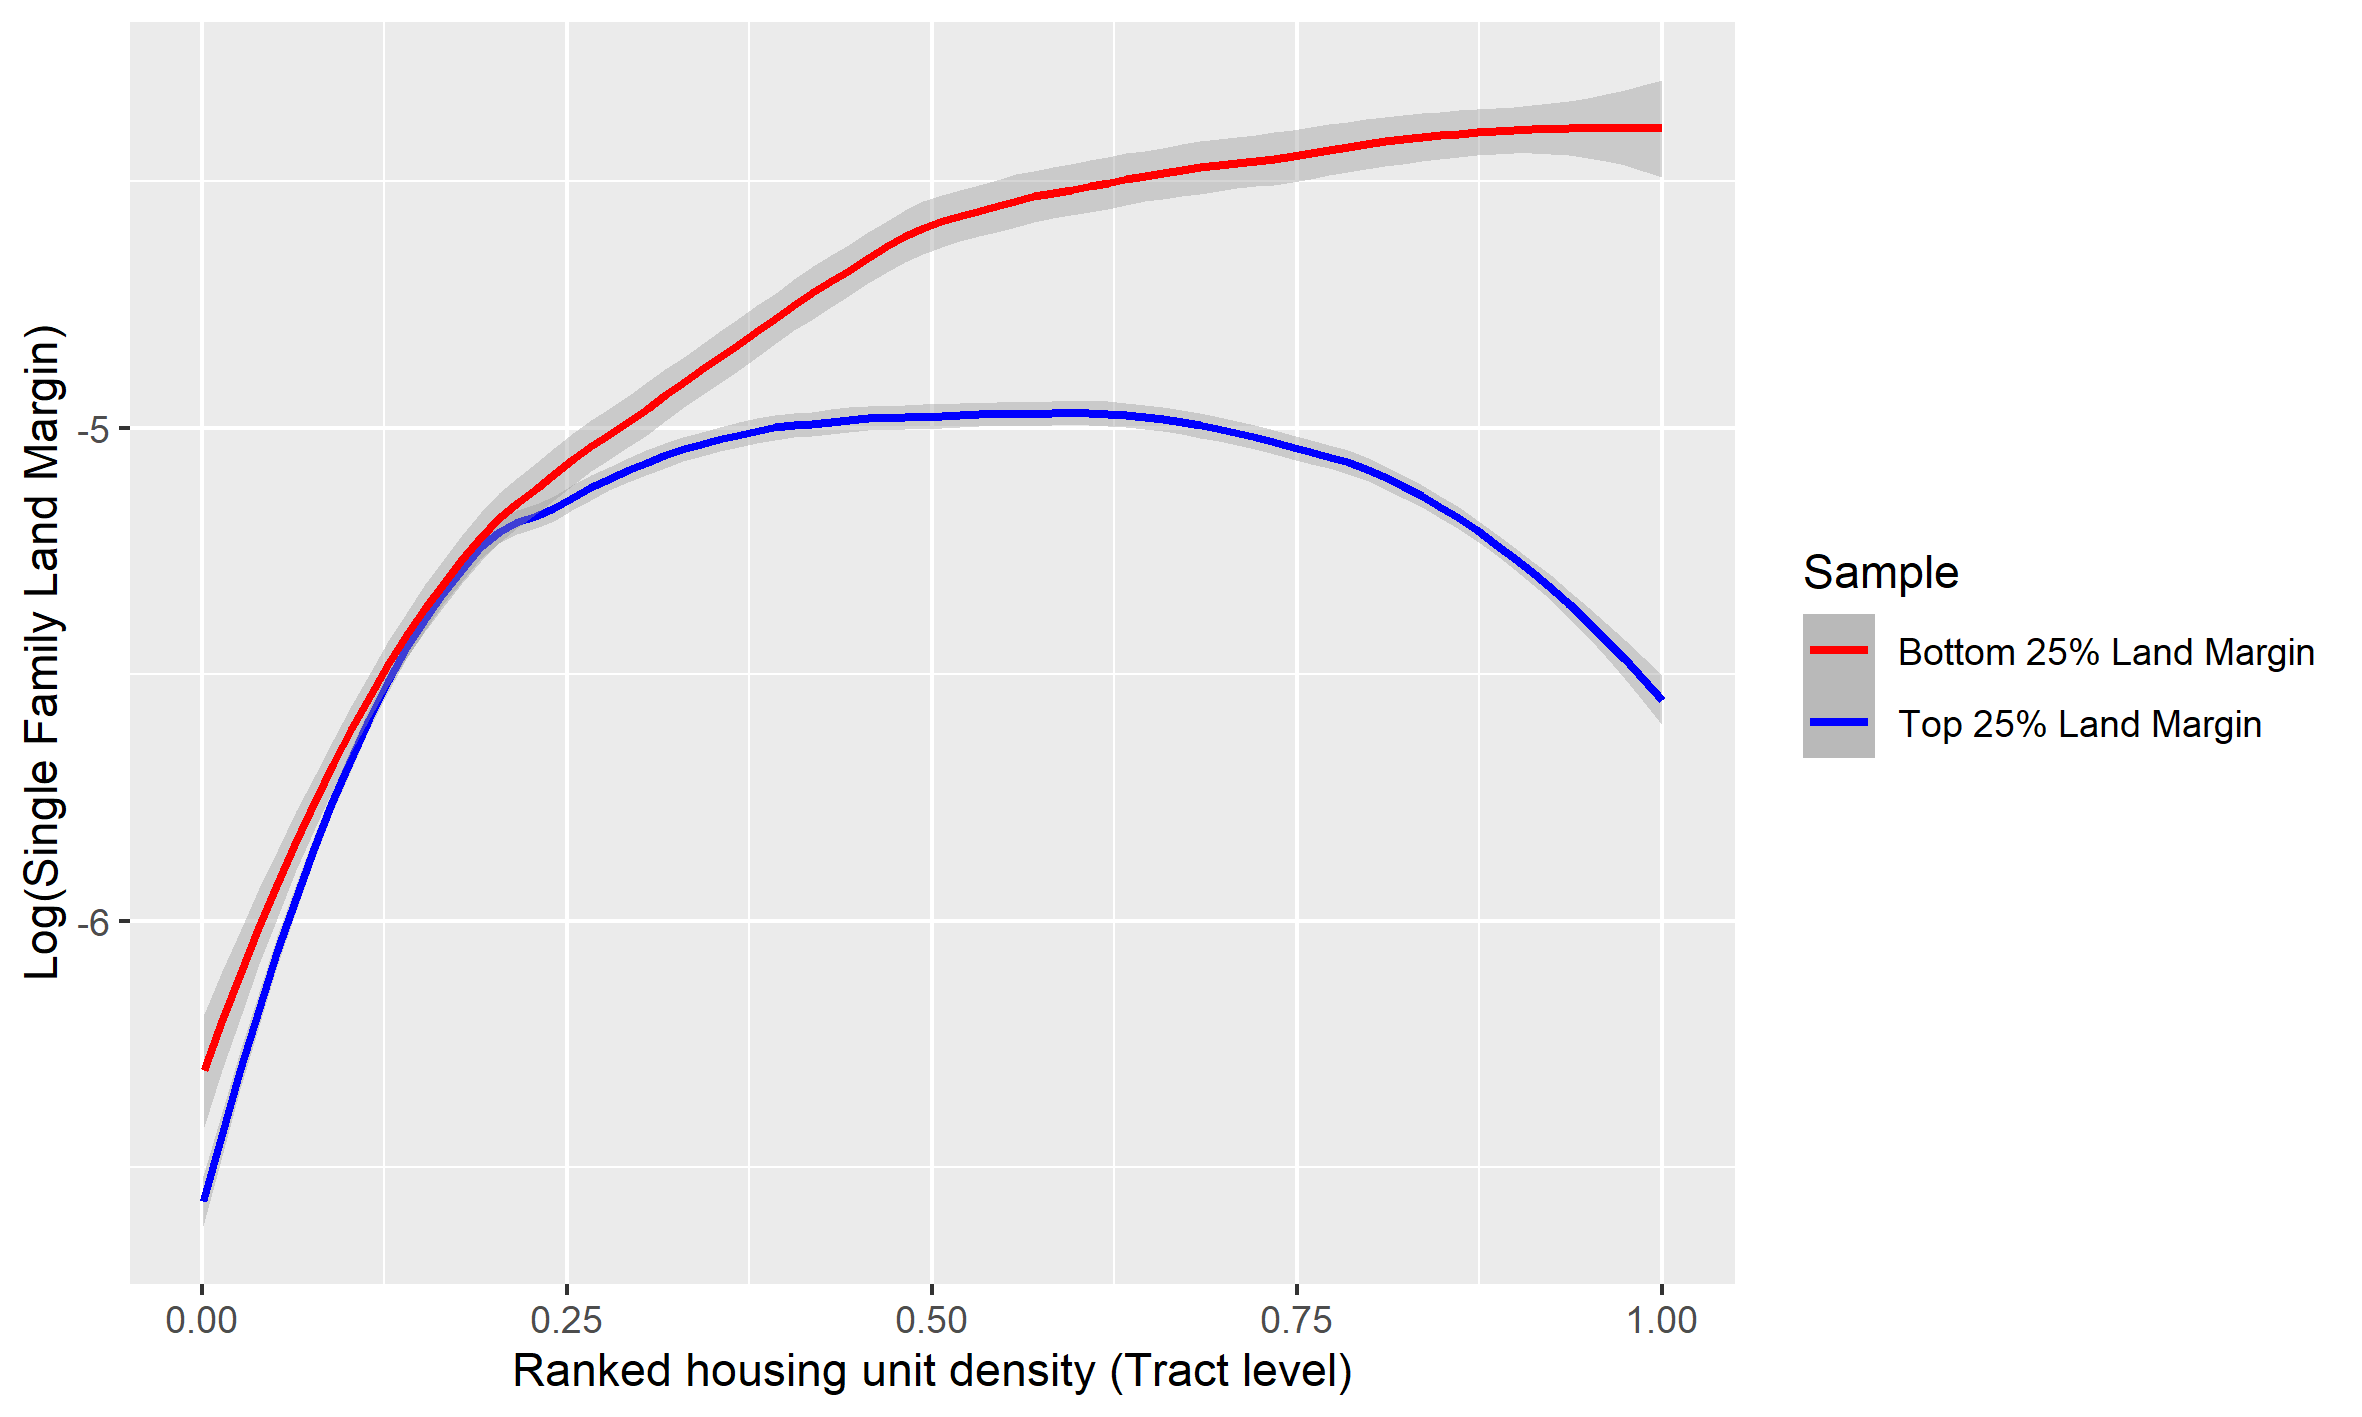
\includegraphics[width=0.7\textwidth, height=0.5\textheight]{SingleFamilyLand.png}}

\end{frame}


\begin{frame}{Appendix: Fact 1 replication with French Data \hyperlink{return}{\beamerbutton{Return!}} }
	\label{3}
	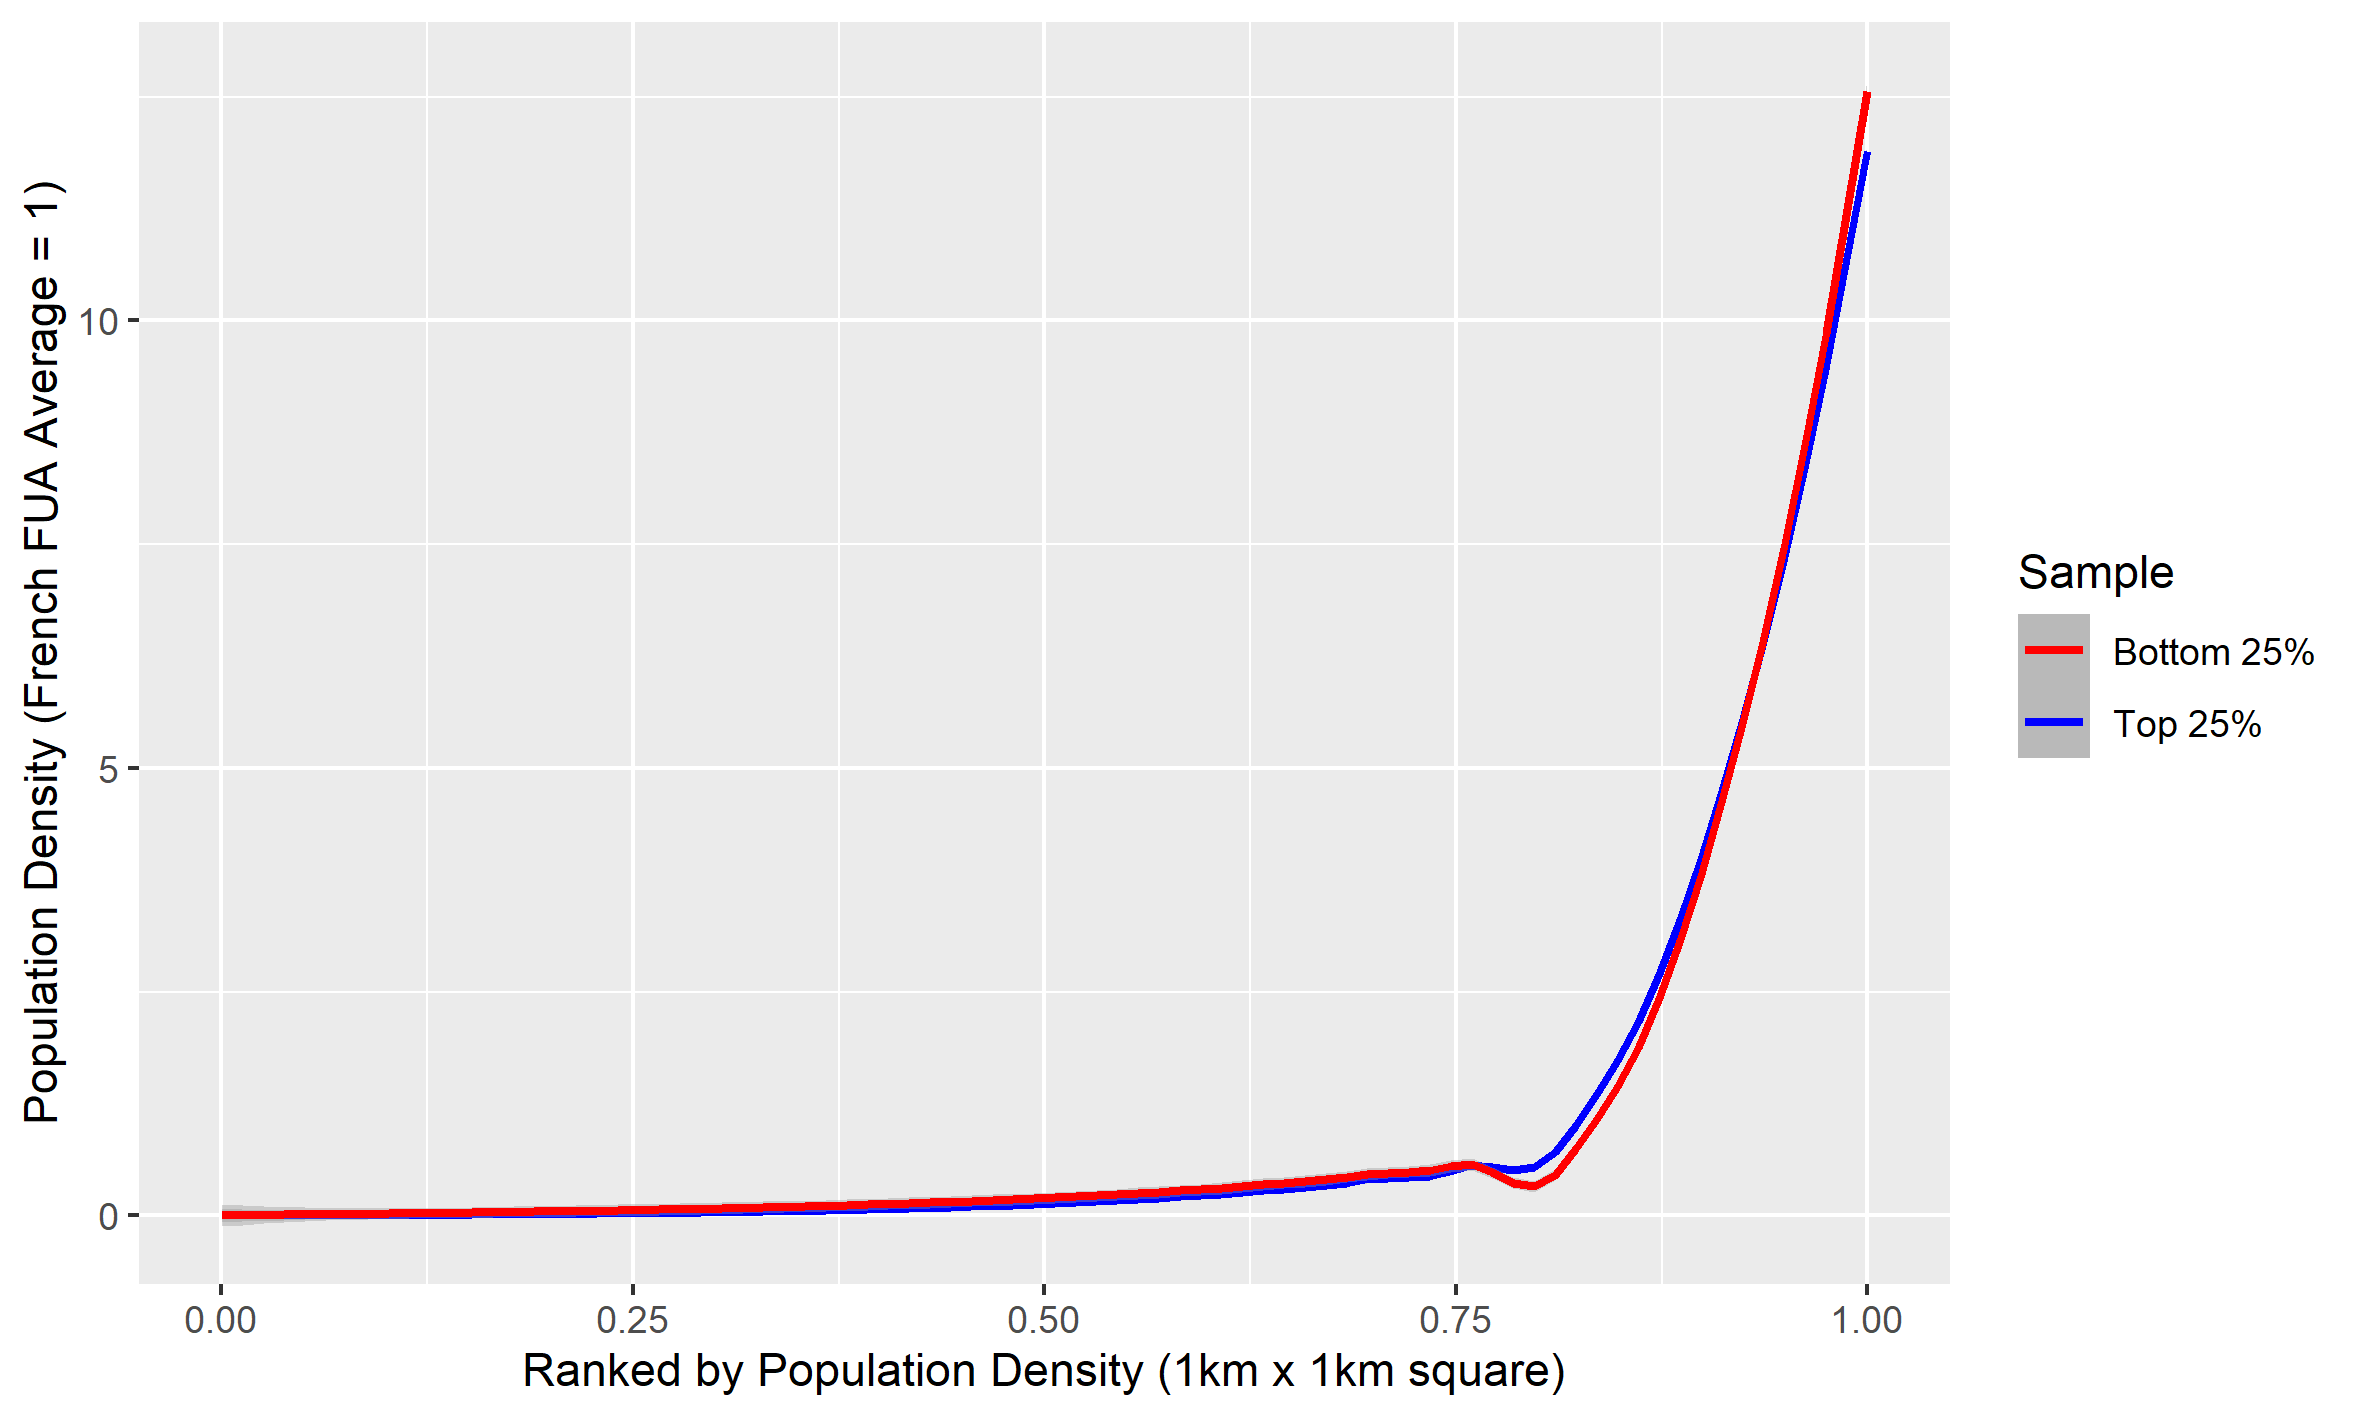
\includegraphics[width=\textwidth]{tractdens_dist_france.png}

\end{frame}

\bibliography{references.bib}
\end{document}